\documentclass{article}
\usepackage{graphicx} 

\begin{document}


\section*{Abstract}
Classification of high dimensional data is always a great challenge because of
``small n, large p'' or ``the curse of dimensionality'' like problems.
To classify high dimensional data simply as it is is not feasible because
none of existing classifiers can handle even tens of thousands in magnitude of
dimentions. So we need to use some sophisticated methods in order to work with
high dimentional data. First, we need method to drastically reduce dimentionality.
Second, there is a natural need to identify stable subset of features that would be
user for classification. Third, we need a technique that would be fast and
scalable. And the ultimate goal is to have a good classification performance. 

\section{Introduction}
\subsection{Subtitle}

A feature subset selection is a task of choosing a small subset of
features that ideally is necessary and sufficient to describe the target concept.

\subsection{Another subtitle}

More plain text.

\section{Experiments and Results}

\subsection{Data Sets}

We user colon data set.

\subsection{Experimental Setup}

For classification we used linear SVM

\subsection{Results}

moo. 

\begin{figure}[htb]
\begin{center}
\leavevmode
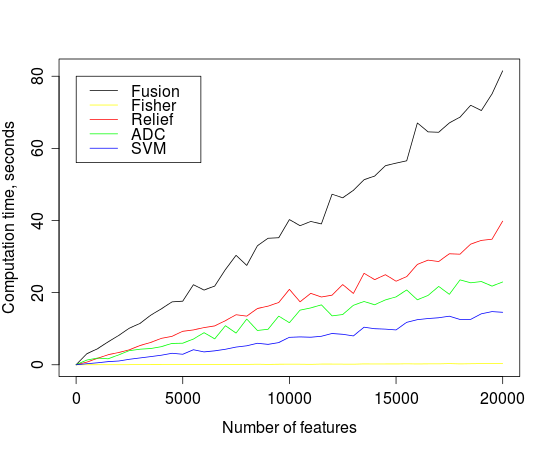
\includegraphics[width=0.5\textwidth]{images/all_performance.png}
\end{center}
\caption{Feature selection speed performance of various methods.}
\label{fig:flash}
\end{figure}

\begin{figure}[htb]
\begin{center}
\leavevmode
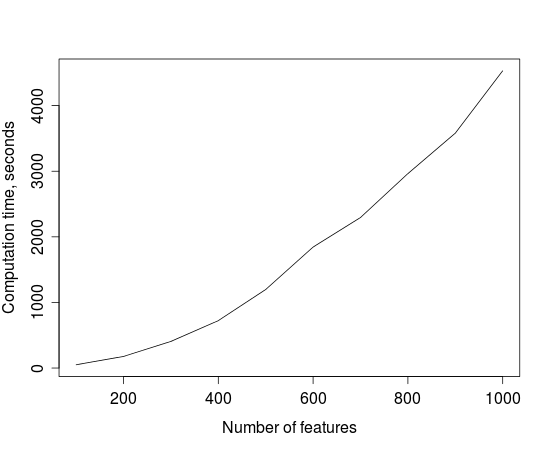
\includegraphics[width=0.5\textwidth]{images/cgs_performance.png}
\end{center}
\caption{Conensus groups stable feature performance.}
\label{fig:flash}
\end{figure}

\end{document}
